\subsection{Introdução}

Em colisões entre íons pesados(íons de chumbo ou ouro) a uma energia da ordem de $100 GeV$ no sistema de referência do centro de massa, é possível obter um novo estado da matéria, chamado de Plasma de Quarks e Gluons, onde estas partículas deixam
de estar confinadas em hadrons, introduzindo novos graus de liberdade no sistema. A temperatura necessária para formar este estado da
matéria é da ordem  de $200 MeV$\cite{letessier_hadrons_2002} ou $10^{12} K$, e a densidade de energia excede o valor típico hadrônico de
$1 GeV/fm^{3}$. As propriedades deste estado da matéria podem ser estudadas analisando os produtos dessa colisão após o resfriamento da
matéria. Através do espectro de $p_T$ das partículas, por exemplo, obtém-se informações sobre a
entropia e a temperatura do plasma, através da multiplicidade das partículas produzidas\cite{letessier_hadrons_2002}.
Em geral, essas propriedades referentes à expansão hidrodinâmica do plasma estarão associadas
ao espectro na faixa de $p_T \approx 0-2 GeV/c$. Na faixa $p_T > 2 GeV/c$, observa-se os efeitos de fenômenos de {\it hard
scattering}. Esses fenômenos são resultado da formação de partículas de alta energia que atravessam o plasma aquecido, depositando
energia neste. Na sua saída, devido às propriedades\cite{skands_introduction_2013} da QCD\footnote{QCD ou {\it Quantum Chromodynamics}
é a teoria que descreve as interações fortes.}, essas partículas se fragmentam criando os chamados jatos ou {\it jets}. Esses jatos sofrem efeitos estruturais por conta da interação dos partons
iniciais\cite{lokhtin_angular_1998,bass_systematic_2009,connors_review_2017,nattrass_jet_2018,denterria_jet_2009} com o plasma.

%\begin{figure}[!h]


 \centering
 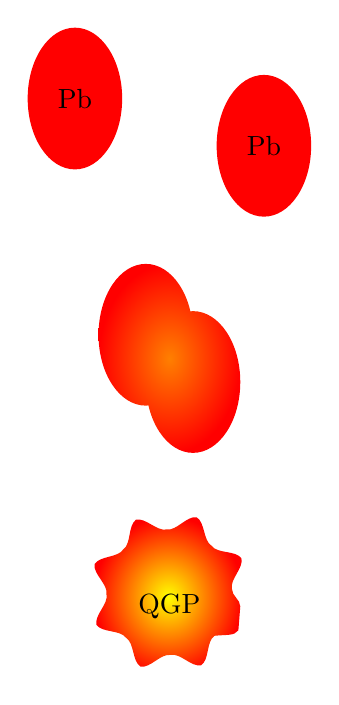
\begin{tikzpicture}[thick,scale=.3]

\fill[red] (0,23) ellipse (2 and 3) node [black,scale=1] {Pb};

\fill[red] (8,21) ellipse (2 and 3) node [black,scale=1] {Pb};

\shade[outer color=red,inner color=orange] (3,13) ellipse (2 and 3) -- (5,11) ellipse (2 and 3);

\shade[inner color=yellow, outer color=red,decorate,decoration={snake,amplitude=3,segment length=20}] (4,1.5) circle (3) node [scale=1] {QGP};

\end{tikzpicture}
\caption{Sequência temporal de colisão de íons pesados.}
\label{qgp}
\end{figure}

Nos instantes iniciais das colisões entre íons pesados, quarks pesados podem ser gerados. Quarks pesados, como o \emph{bottom}, podem ser utilizados como ponta de prova para o estudo do Plasma de Quarks e Gluons
devido à sua interação com este em seu caminho para fora da região de interação\cite{li_inverting_2017,renk_jet_2014}. Eles
interagem com o meio de duas formas, através da radiação induzida, ou \emph{gluonsstrahlung}, e através de reações colisionais.
Embora estes mesmos efeitos ocorram para quarks leves, a massa dos quarks pesados limita a sua perda de energia e também sua
velocidade\footnote{Especialmente no limite $E \approx m$}, o que permite que ele ``colete'' mais informações sobre o QGP,
uma vez que, tendo menor velocidade, o quark passa muito mais tempo dentro do plasma\cite{renk_jet_2014}.

\subsection{Objetivo}

O objetivo deste trabalho é investigar como diferentes modelos tratam os efeitos da expansão do meio formado em colisões
entre íons pesados relativísticos na estrutura de jatos formados pela fragmentação de quarks pesados. Diversos modelos serão
investigados e, após uma avaliação dos mesmos, pretendemos implementar em um ou mais modelos uma descrição mais detalhada desse meio,
considerando-se flutuações evento por evento e eventualmente, outras características do meio, como sua viscosidade. Posteriormente,
observaremos a distância angular entre os centros dos subjatos e a fração energética compartilhada entre ambos.
Certos modelos \cite{zapp_monte_2009, renk_jet_2014} preveem que o meio deve interferir em processos de perda de energia.

\subsection{Métodos}

Para a realização desse trabalho utilizaremos geradores de eventos, que são essencialmente simuladores
de colisões hadrônicas, para verificar os efeitos esperados do meio hidrodinâmico em expansão na fragmentação
de quarks pesados, que podem ser observados através do estudo da subestrutura de jatos. Os programas que serão
investigados são:

\begin{itemize}
 \item v-USPhydro\cite{noauthor_jacquelyn_nodate,noronha-hostler_event-by-event_2016,noronha-hostler_bulk_2014,noronha-hostler_sensitivity_2016},
 modelo relativístico de fluxo hidrodinâmico(2+1) com viscosidade;
 \item JEWEL\cite{noauthor_jewel_nodate, zapp_jewel_2014}, constitui um gerador de eventos com modelos específicos de \emph{Jet Quenching};
 \item PYTHIA\cite{noauthor_pythia_nodate}, que constitui em um gerador de colisões próton-próton;
 \item MUSIC\cite{noauthor_music_nodate};
 \item HYDJET\cite{lokhtin_hydjet++_2009}, constitui um gerador de colisões hadrônicas combinado com um algoritmo de simulação hidrodinâmica;
\end{itemize}